\documentclass[letterpaper,10pt,a4paper]{article}
\usepackage{ulem}
\usepackage{url}

\usepackage{epsfig}
\usepackage{graphicx,color}% Include figure files
\usepackage{wrapfig,caption}
\usepackage{epstopdf}

\usepackage{fancyhdr,graphicx,epsfig,lastpage}
\usepackage{amsmath}
\usepackage{amssymb}

\usepackage{latexsym}
\usepackage[latin1,applemac]{inputenc}

%\usepackage{natbib}



\usepackage{mdwlist}
%\usepackage{enumitem}

%\usepackage[sort&compress,sectionbib]{natbib}
% \usepackage{german,isolatin1}
\usepackage{indentfirst}
%\usepackage{natbib}

\setlength{\parindent}{0in}
%\usepackage[superscript]{cite}

\usepackage{setspace} % Allows spacing of sections with \singlespacing and \doublespacing command

\oddsidemargin 0pt 
\evensidemargin 0pt 
\marginparwidth 68pt 
\marginparsep 10pt 
\topmargin 0pt 
\headheight 10pt 
\headsep 5pt

\voffset -40pt 
\footskip 35pt 
\textheight 23cm 
\textwidth 16.8cm 
\columnsep 10pt 
\columnseprule 0pt 
\sloppy 
%\frenchspacing

\linespread{1.27}

%\setlength{\parindent}{0pt} 
%\setlength{\parskip}{5pt plus 2pt minus 1pt}
%\renewcommand{\baselinestretch}{1.095} %{1.2} %{1.095}
%\clubpenalty=5000 \widowpenalty=5000
%\renewcommand{\footnoterule}{\vspace{0.5cm}%
%  \rule{2.5in}{0.4pt} \vspace{0.3cm}} \pagestyle{fancy}
%\renewcommand{\headrulewidth}{0.4pt} \lhead{Research Plan} \chead{}
%\rhead{\today} \renewcommand{\footrulewidth}{0.4pt} \lfoot{}
%\cfoot{\thepage /\pageref{LastPage}} \rfoot{}

%%%%%%%%%%%%%%%%%%%%%%%%%%%%%%%%%%%%%%%%%%%%%%%%%%%%%%%%%
% Main
%%%%%%%%%%%%%%%%%%%%%%%%%%%%%%%%%%%%%%%%%%%%%%%%%%%%%%%%%
\begin{document}
%\noindent
\begin{center}

  %\textbf{\Large Research Plan}\\[10mm]

%  \textbf{Title:}\\[5mm]
% \textbf{\Large Measuring Incentives for Attacks \& Security, }\\[4mm]
% \textbf{\Large and Managing Cyber Risk}\\ [10mm]

  %{\today}\\[85mm]

  %\textbf{PhD candidate:}\\
 % \textbf{\large Thomas Maillart}\\[10mm]

  %\textbf{Advisor:}\\
  %Prof. Dr. Didier Sornette\\
  %Chair of Entrepreneurial Risks\\
  %ETH Z\"urich (Swiss Federal Institute of Technology in Z\"urich)\\[5mm]

  % \textbf{Co-referee:}
  % \\[5mm]
  

\vspace{-0.5cm}
{\Large {\bf \textsc{Bringing Order to Wikipedia with Bi-Partite Network Rankings\\�}}}

\vspace{0.2cm}
{\large {\bf \textsc{Maximilian Klein, Thomas Maillart, John Chuang}}}
\vspace{0.15cm}
\end{center}

%Open source software has been one of the most successful incarnations of open innovation, providing considerable amount of software code as a public good for the development of reliable Internet and Web infrastructures, operating systems, and a broad range of applications.  Moreover, open source software (OSS) has inspired many initiatives beyond software development, such as Wikipedia  which combines (i) task self-selection and (ii) peer-review by participants.
\vspace{0.05cm}
%{\Large \bf Research Interests} \vspace{0.25cm}\\


%\clearpage
%\bibliography{../tmaillart.bib}

From open source software projects to online encyclopedias, open collaboration has become one of the greatest successes of the Internet, with millions of individuals sharing knowledge as a collective good. \cite{vonhippel2003oss}. One way that these projects are successful is that they can capture the efforts of the most highly active users - {\it power-users} - just as well as the smaller users. \cite{ The long tail or similar} When it comes to the the quality of the final product, we would like to know how important power-users are to success.
Specifically here, we tackle the problem of characterizing how heavily a Wikipedia category is controlled by power users.

The category level has been described as the {\it meso-level} of Wikipedia, and can be viewed as a bi-partite network between editors and articles \cite{jesus2009}. 

Performing calculations on the bi-partite network as model has been proposed in Economics to rank countries and products \cite{hidalgo2009}, and the method has been shown to be able to predict GDP. \cite{caldarelli2012network}.

In the Wikipedia bi-partite network, we adopt the premise that the quality of an editor depends on the size and quality of the portfolio of touched articles. And that the quality of an article depends on the size and quality of the log of touching editors. Although this many seem circular a solution is available \cite{caldarelli2012network}

Therefore we borrow their quality metric $\mathbf{w^*}$ for editors $e$ and articles as $a$ defined by:
\begin{equation}
\begin{cases}
w^{*}_{e} \sim k^{1-\beta}_{e} \langle k_{a}^{-\alpha}\rangle_e \\
w^{*}_{a} \sim k^{1-\alpha}_{a} \langle k_{e}^{-\beta}\rangle_a
\end{cases} \label{eqsim}
\end{equation} 

Where $k_e$ is the number of articles touched by editor $e$, and $k_a$  is number of editors touching article $a$. Similarly $\langle k_{a}^{-\alpha}\rangle_e$ is the arithmetic average of $k_{a}^{-\alpha}$ the articles touched by editor $e$, and $\langle k_{e}^{-\beta}\rangle_a$ is arithmetic average of $k_{e}^{-\beta}$ the editors touching article $e$.

Meanwhile we calculate state of the art ground truth exogenous ranks $v_e$ and $v_a$ which are labour hours of editors \cite{geiger2013}, and a suite of text analysis measures on articles \cite{wang}.

----------

Despsite the calculation appearing to be circular, it can be solved recursively. The quality of editors and articles can be viewed as a heatmap of most touched nodes on a random walk along the bi-partite network of editors and articles shown on Figure \ref{fig1}A. We can tune our models by the probabilities of landing on more ubiquitously edited articles, and more diversified editors, by variables we call $\alpha$ and $\beta$. Therefore when we maximize the correlations between the ranking given by the bi-partite model, and standard metrics of editor and article quality, we find the most characteristic measurements of a category given by $\alpha$ and $\beta$.
----------



\begin{figure}[h]
\centering
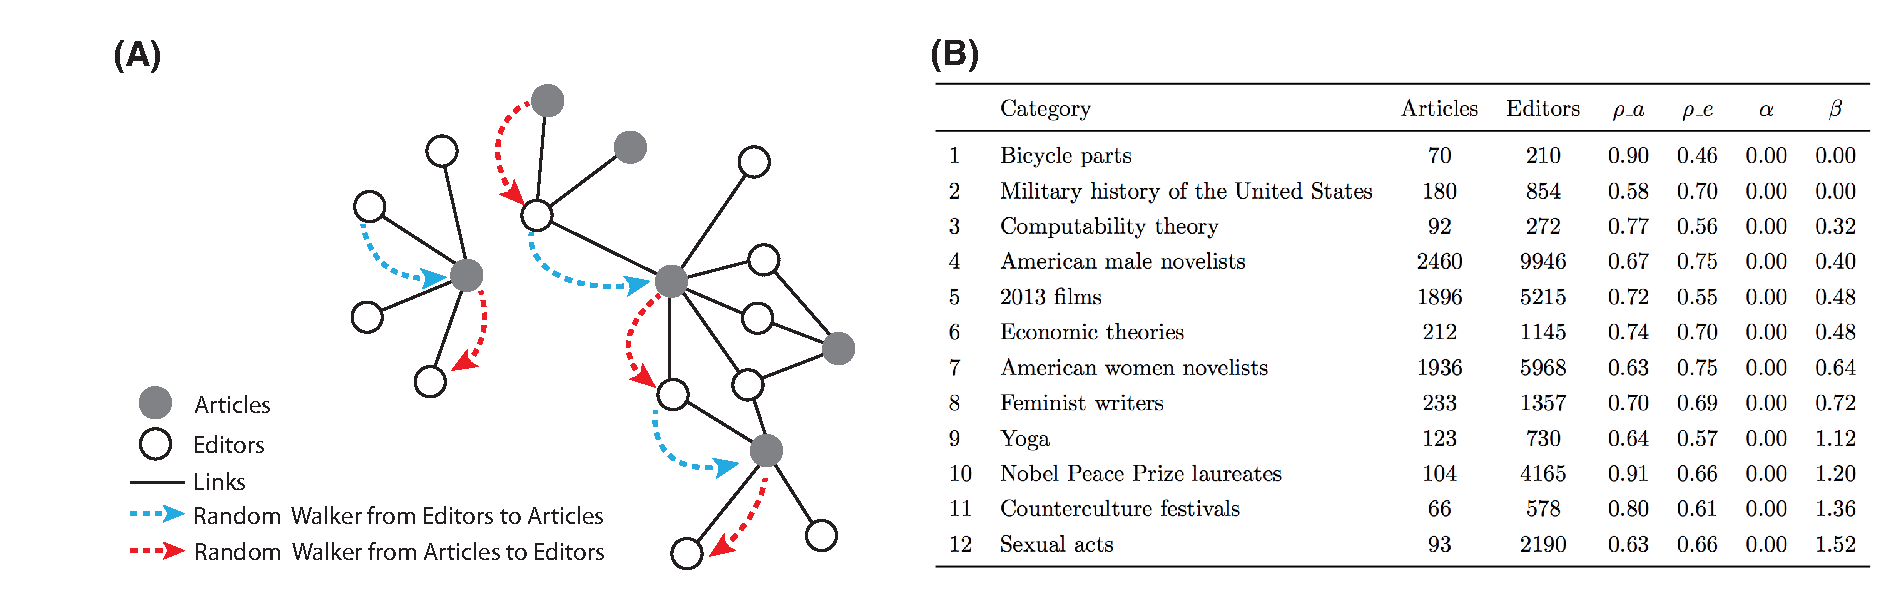
\includegraphics[width=0.8\columnwidth]{Figures/figure_abstract.eps}
\caption{{\bf (A)} Bi-partite network with Article and Editor nodes. Dashed arrows show how the random walker jumps from one node to another type of node with some probability controlled by the appropriately biased connectivity of the each node. {\bf (B)} Table shows the best rank-correlation $\rho_a$ and $\rho_e$ of the algorithm with the ground truth for each Wikipedia category, as well the value of the bias $\beta$.}
\label{fig1}
\end{figure}

We calibrate our model by finding values of $\alpha$ and $\beta$ that maximally correlate the rank produced by the bi-partite network and the exogenous ranks. We achieve high correlations around $0.7$  which means that we may turn to see what values of  $\alpha$ and $\beta$ caused this correlation and what it means as an exhibited behaviour of those categories.

The most notable result is in correlating article rankings there is a very clear solution space along $\alpha = 0$ across all categories. Namely that article quality is mostly explained as a simple count of contributing editors.  

We would like to find solutions which maximize editor and article ranking correlations simultaneously so we could make a complete statement about all aspects of the category. We search the solution space of editor ranking correlations along $\alpha = 0$, whose interpretation in editor ranking is that the quality of articles in their edit portfolio is inconsequential. For each category we find different maximizing values of $\beta$, which is a measure of importance of portfolio size. High $\beta$ means that portfolio size is less important for successful editors, and vice-versa, low $\beta$ means article diversity counts more.

Looking at \ref{fig1}B, we find interesting extremes. The best editors in {\it Category:Military history of the US} - a category known for being very competitive -  are characterized by emphasizing their article portfolio size. On the other end, the editors in {\it Category:Sexual acts} - a taboo subject where much editing could be considered perverse - are characterized by de-emphasizing their portfolio size in the category.

Now if we allow that portfolio size, the number of articles that an editor has touched, is a proxy for a power-user, then our $\beta$ measure is an indicator for power-user domination of a category. Therefore using this method, open collaborations online can detect the importance of power-users to a specific project. 




%While wikiRanks incorporates only bi-partite links input information, we find high rank correlations ($\rho = 0.7\pm0.1$) with usual Wikipedia editors' expertise and articles' quality metrics. The wikiRanks algorithm also provides deep insights on the structure of online collaboration. We find that editors in some categories of Wikipedia articles achieve more quality with a large number of editors per article, while for other categories, quality is more achieved as a result of expertise of editors.





\clearpage
\vspace{1cm}
\bibliographystyle{abbrv}
\bibliography{sigproc,tmaillart}  


\end{document}

%\vspace{3cm}
%
%
%However, the potentially large number of participants with various engagement levels generate non-linear contribution dynamics as a result of complicated interaction feed-back loops. These {\it productive bursts} raises outstanding challenges for management -- in particular overload and illusion of control , which might in turn impede the desired innovation process. Hence rather than controlling, our recent research suggeasts the manager should steer the community towards her goals according to the principles of open innovation organizational design \cite{vonKrogh2012cmr}. However, to be enforced, these principles still require close monitoring and even forecast by the manager to react and adapt the ``game" rules. Fortunately, nowadays large parts of open innovation ventures are mediated through Internet platforms that record big data on user contributions and behaviors. And unfortunately, managers currently lack metrics to monitor, forecast and adequately organize and steer open innovation as a collective action of interacting individuals with heterogenous motives.\\
%
%Building on research in  physics of complex systems, quantitative sociology and economics, and in particular on our research on :
%
%\begin{itemize}
%\singlespacing
%  \item self-organization of knowledge reuse as a {\it rich-get-richer} effect \cite{maillart2008},
%  \item economic origins of long-memory processes in human timing \cite{maillart2011},
%  \item collective dynamics of open source software (OSS) production \cite{maillart2011wp,maillart2011mechanisms},
%  \item machine learning and predictability of contribution epidemics in OSS \cite{pautex2012},
%  \item the effects of diversity of open source licenses and cumulative innovation \cite{maillart2012osslicenses},
%\end{itemize}
%
%I propose to investigate the mechanisms of interactions and self-organization in open innovation, with the goals to understand the conditions of collective action emergence in society \cite{ostrom1990} and to provide managers with tailored tools to successfully implement and organize open innovation. 
%
%\vspace{1cm}
%{\bf a. Exogenous vs. Endogenous Dynamics of Contributions and Social Interactions}\\
%A class of models is particularly suitable to investigate social processes, especially when taking into account long-memory of human timing \cite{maillart2011}. Initially, proposed by Hawkes \cite{hawkes1971b,hawkes1971}, the conditional Poisson process can be regarded as the generalization of the non-homogeneous Poisson process, whose intensity $\lambda(t)$ defined such that $\lambda(t)dt$ is the expected value of the number of events in the time interval $[t,t+dt)$, depends not only on time $t$ but also on the history of the process according to
%
%\begin{equation}
%\lambda(t) = \mu(t) + \sum_{t_i < t} h(t-t_{i}),
%\label{monoexcited}
%\end{equation}
%
%where $t_i$ are the time stamps of past events, $\mu(t)$ is the background intensity, and $h(t-t_{i})$ is the memory kernel function that weights how much past events influence future generations of events and controls the amplitude of endogenous feedback mechanisms, i.e. how many daughters events an initial exogenous shock will trigger. As initially proposed by Hawkes \cite{hawkes1971}, formula (\ref{monoexcited}) generalizes into a multivariate process \cite{liniger09}, which is well-suited to capture interactions between various processes such as streams of programmers' work in OSS projects and to what extent the mutually excite \cite{saichev2012}. While the mono variate version of the self-excited point process has been repeatedly found to be a robust model in various socio-economic systems such as open source software \cite{maillart2011wp} and social networks \cite{crane2009}, the multi-variate method has only been used to model contagion across financial markets \cite{ait-sahalia2010} and interactions between cyber attacks \cite{baldwin2012}. To perform calibration in high dimensional social systems (i.e. with large groups of contributors), this method requires important amount of data to capture enough signal. Therefore, this method shall be well suited for testing with big data of open source software repositories. 
%
%
%
%\vspace{1cm}
%{\bf b. Managing Cooperation, Free-Riding and Conflicts}\\
%Current research on open source is generally highly biased in favor of open source: on the contrary to common wisdom developers do not only cooperate, they also free-ride and defect. The open source community is regularly shaken by conflicts that weaken or even simply endanger projects. Beyond providing a more balanced view of research on success of open innovation, studying conflicts in open source software is an opportunity for research and for management. Attributing a cost to social interactions, it is possible to reverse engineer scenarios of cooperation, free-riding and conflict directly from time series, and to rationalize them in the game theory framework. While quantification of interaction intensity can be directly extracted from activity time series, the challenge consists in identifying the reasons of cooperation and conflicts between individuals and groups of individuals. For that two options are possible: (i) extract emotions expressed on development forums \cite{mitrovic2010} and/or (ii) characterize the nature of interactions directly from content of contributions. For instance, if a developer systematically deletes the work of others, this might be a signal of conflict. Furthermore, exploring the dynamics of interactions can help understand and model how conflicts arise and how they are eventually resolved either by involving third party mediators or bargaining on produced content. This work package shall be seen as an extension of Granovetter's strength of weak ties to the time dimension \cite{granovetter1973}.
%
%\vspace{1cm}
%{\bf c. Bi-Partite Networks of Knowledge Production}\\
%Open innovation occurs with unpredictable engagement and various input quality. However, a large stream of management literature has described progressive integration of individual to projects (i.e. the {joining script}) as meritocratic process by which contributors demonstrate increase of expertise to approach the development core at the top of the hierarchy \cite{vonKrogh2003}. However apart for source code that can be compiled, executed and {\it hardware} benchmarked \cite{gulley2010}, knowledge value cannot directly be assessed and {\it a fortiori} individual contributions cannot be easily disentangled. Indeed, an endogenous reinforcing process occurs between social status and quality of production. Characterization, measurement, modeling and calibration of this endogenous ``growth" process through bi-partite networks of producing entities with specific skills and products \cite{hidalgo2009} provides rich insights and predictions capabilities of individual work as a contributing part of the collective production process \cite{maillart2012b}. 
%
%\vspace{1cm}
%{\bf d. Emergence and Sustainability of Hierarchical Organizations}\\
%The open source community and to some extent related literature \cite{raymond1999} has praised the {\it bazaar} organization of open source projects. In 2002, Benkler proposed that peer-production should be a third way of production organization \cite{benkler2002}, besides market and firm as theorized by R. Coase \cite{coase1937}. The main argument for extending Coase's theory of transaction costs as a driver for the emergence of firms was that the Internet provides communication capabilities at negligible costs. Yet communities tend to self-organize to cope with internal inefficiencies and therefore spontaneously recreate various levels of hierarchies. A vivid example of this phenomenon is Wikipedia: while modifications on any page was initially allowed to anyone, some barriers have been progressively raised to protect articles against defacement and to ensure quality. Nowadays, Wikipedia is a well structures open source project, which requires contributors to follow a precise {\it joining script}.  This suggests that open innovation can have various degrees of organization ranging from market (i.e. peer transactions in production ) to firm (i.e.principal-agent configuration) as a function of time, number of developers, complexity of work to achieve, etc. Armed with the tools developed to monitor, characterize, and model open source production and social interactions at work in open source projects, and the capabilities to measure transaction costs between developers, I finally propose to test the Coase's theorem in the context of open innovation, by data mining social interactions and production details of thousands of open source projects, and by identifying and extracting transaction costs between contributors or groups of contributors.

%%%%%%%%%%%%%%%%%%%%%%%%%%%%%%%%%%%%%%%%%%%%%%%%%%%%%%%%%